\documentclass[../notes.tex]{subfiles}

\pagestyle{main}
\renewcommand{\chaptermark}[1]{\markboth{\chaptername\ \thechapter\ (#1)}{}}
\setcounter{chapter}{5}

\begin{document}




\chapter{Intro to Long Reports}
\section{Lecture 10: Scientific Visual Communication}
\begin{itemize}
    \item \marginnote{2/7:}Long report submissions delayed until Friday.
    \begin{itemize}
        \item The content of today may be useful!
    \end{itemize}
    \item Thursday.
    \begin{itemize}
        \item Anna Wuttig on the current state of EChem.
        \item Tokmakoff will stick around after for us to chat about our reports with him.
    \end{itemize}
    \item There are many aspects beyond \emph{visual} communication, but this is one that isn't always seen, so Tokmakoff decided to focus on it today.
    \item Take all the guidelines and extra chapters seriously; they're exactly what is being graded for.
    \item We should care about communication because it's as important to our career development as anything.
    \begin{itemize}
        \item Our science must be distributed; otherwise, we're just a hobbyist.
    \end{itemize}
    \item We need to convey very complicated, quantitative information to other scientists, management, government agencies, policy makers, investors, and the general public.
    \item Reduce complex quantitative data accurately into \underline{clear, concise} messages: Data interpretation.
    \item Often, there are real requirements on content and formatting.
    \item Excellence in communication.
    \begin{itemize}
        \item Content is key, but saying it well will really level you up.
        \item It develops \emph{trust} in your methods, results, and communications.
        \item A well-communicated report and graphic can change the world, e.g., the hockey stick curve.
    \end{itemize}
    \item \textbf{Communication}: The means of exchanging information.
    \item \textbf{Medium}: Any channel of communication.
    \item Media we will discuss.
    \begin{itemize}
        \item Print (text, graphics).
        \begin{itemize}
            \item Graphics are how people digest scientific information.
        \end{itemize}
        \item Oral (in person with visual support).
        \item Never use double columns if you want transport to online.
    \end{itemize}
    \item The common starting point for all communication.
    \begin{enumerate}
        \item Audience.
        \begin{itemize}
            \item Identify; sets the objective, expectations, language, and aspects of your work to focus on.
            \item You need to know if you're talking to fellow bench scientists, or senior management.
        \end{itemize}
        \item Message.
        \begin{itemize}
            \item What are you trying to say? Just say what you need to, and get rid of the rest.
            \item When your TA or Tokmakoff reads your report, what are they going to think of my magenta line.
        \end{itemize}
        \item Media.
        \begin{itemize}
            \item What tools are at your disposal, and how are they best employed.
        \end{itemize}
    \end{enumerate}
    \item Visual presentation tips for text and graphics.
    \begin{itemize}
        \item Our goal: Communicate quantitative information clearly and concisely.
        \item Make your viewer's life easy (be consistent, define the purpose of each element, etc.).
        \item Simplicity is good; clutter is bad.
        \item Color should be chosen with a real focus in mind.
    \end{itemize}
    \item Typefaces and fonts.
    \begin{itemize}
        \item The visual representation of language. Its style should help, not interfere, with your communication.
    \end{itemize}
    \item \textbf{Typeface}: The design elements for lettering. A collection of glyphs.
    \item \textbf{Glyph}: A single representation of a character.
    \item \textbf{Font}: A variation of a typeface like size, weight, and spacing.
    \item Classes of typefaces: \textbf{Serif} and \textbf{sans serif}.
    \begin{itemize}
        \item Sans-serif is good for titles, headings, and labels.
        \item Serifs are good for presenting large amounts of text.
    \end{itemize}
    \item History of typefaces.
    \begin{itemize}
        \item Use legacy typefaces; they're still supported.
        \item "Microsoft is your friend."
        \item Computers revolutionized typography; Microsoft drove the development with proprietary stuff, which eventually caused them to lose the edge, and now there's great open-source fonts.
    \end{itemize}
    \item Typefaces for equations.
    \begin{itemize}
        \item Times New Roman and Garamond have full math support.
        \item Computer modern (\TeX) is probably still the best in terms of being able to distinguish things since it includes so many helpful flourishes.
        \begin{itemize}
            \item You're probably encountered difficulties with the lab manual (e.g., $v$ vs. $\nu$) because it's not in Computer modern.
        \end{itemize}
    \end{itemize}
    \item Tokmakoff's recommendations for formatting: Typed $8.5\times 11$ documents should have a\dots
    \begin{itemize}
        \item Single column format.
        \item $1''$ margins.
        \item 11-12 point type.
        \item $\sim 90$ characters per line including spaces (15 characters per linear inch).
        \item 4-5 lines per vertical inch.
    \end{itemize}
    \item Why worry about font size?
    \begin{itemize}
        \item Legibility vs. readability; too small impacts legibility, and too big impacts readability.
    \end{itemize}
    \item Why worry about line spacing?
    \begin{itemize}
        \item $1.5\times$ is Tokmakoff's recommendation.
        \item $2\times$ is legacy from typewriters, when single and double were the only options.
    \end{itemize}
    \item Why worry about margins?
    \begin{itemize}
        \item White space helps with clarity.
        \item Don't just insert figures; make figures break text.
    \end{itemize}
    \item Equations should be numbered.
    \item Color.
    \begin{itemize}
        \item Don't let it distract; let it help you make a cleaner presentation.
        \item Really bright colors draw the eye too much.
    \end{itemize}
    \item Scientific figures.
    \begin{itemize}
        \item Purpose: To convey quantitative information on the relationship between different physical variables with minimal effort.
        \item Each figure should convey information on exactly one topic.
        \item Again, know your audience, be aware of your medium (typed vs. oral), clarity, etc.
        \item Additional consideration for scientific reports: Often the figure is the only documentation of the data.
        \begin{itemize}
            \item If the reader wanted to analyze your data, can they read data values off the graph using the axis labels?
            \item Raw Excel sheets, other records may not be saved, so the literature report may be the only way for future scientists to reanalyze your data.
        \end{itemize}
    \end{itemize}
    \item Examples of good and bad figures.
    \begin{itemize}
        \item As you see scientific figures going forward, take note of what you like and what you don't like and learn.
        \item Tokmakoff asks for the class's feedback on his examples.
    \end{itemize}
    \item You should have 4-6 axis labels and 4-10 tick marks.
    \begin{itemize}
        \item More tick marks than labels is a good idea!
    \end{itemize}
    \item Make sure colors translate to black and white, so maybe I should vary both shapes and colors in my Birge-Sponer plot.
    \item Rowan is very picky about what Excel settings you use.
    \begin{itemize}
        \item Don't cut and paste into word; stuff gets realigned.
    \end{itemize}
    \item Tokmakoff doesn't look for units for unitless quantities (e.g., absorbance).
    \item Use a legend when there are two or more series being plotted.
    \item Caption.
    \begin{itemize}
        \item Use for report figures.
        \item It should describe what is plotted and is needed to interpret the data beyond what is in the figure.
        \item For data, typically quote specific experimental conditions.
    \end{itemize}
    \item Titles are only for oral presentation graphics.
    \item Don't mislead! Rescaling your axes can mislead about growth.
    \item Make everything 300 dpi.
    \item Publishers use JPG in CMYK color profile.
    \begin{itemize}
        \item Online: Use RGB color profile.
        \item Everything else is up to us.
    \end{itemize}
    \item Takeaways.
    \begin{itemize}
        \item Clarity and conciseness.
        \item White space is good!
        \item Microsoft is (mostly) your friend.
        \begin{itemize}
            \item Their templates, colors, and fonts have been professionally designed\dots with everyone in mind.
            \item Use recommended formatting, but be aware it isn't for scientists.
        \end{itemize}
        \item There are no firm rules --- just guidelines. It is an art.
    \end{itemize}
\end{itemize}



\section{Lecture 11: Electrochemistry}
\begin{itemize}
    \item \marginnote{2/9:}Guest lecture by Anna Wuttig.
    \item Ben Masters (our TA) is one of her grad students.
    \item Electrochem can solve important problems, and we know the mechanisms in principle because we can measure the flow of electrons in it as current.
    \begin{itemize}
        \item Thus, we can modify whatever we want and have an \emph{in situ} handle on reaction rate.
        \item This is why it's important for physical chemistry, which seeks to understand, predict, and rationally design future reactions.
    \end{itemize}
    \item We will focus on \ce{CO2}-reduction today.
    \begin{itemize}
        \item Wuttig hopes to \textbf{upconvert} it to other things.
    \end{itemize}
    \item We currently do this with the water-gas shift reaction and Fischer-Tropsch chemistry.
    \begin{itemize}
        \item But this is both energy-intensive and has poor selectivity.
    \end{itemize}
    \item Alternative: Electrochemistry.
    \item Example.
    \begin{equation*}
        \ce{2CO2 + 2H2O <=> C2H4 + 3O2}
    \end{equation*}
    \begin{itemize}
        \item Produces ethylene (used in a lot of things in industry) and \ce{O2} (benign).
        \item Allows you to store $\Delta G=\SI{1343}{\kilo\joule\per\mole}$ of energy, corresponding to $\Delta E=-\SI{1.16}{\volt}$.
        \item This involves two electrochemical half-reactions (recall from gen-chem).
        \begin{align*}
            \ce{2CO2 + 12e^- + 12H+} &\ce{<=>} \ce{C2H4 + 4H2O}\tag*{$E^0=\SI{0.07}{\volt}$ vs. RHE, $\pH=7$}\\
            \ce{2H2O} &\ce{<=>} \ce{O2 + 4e^- + 4H+}\tag*{$E^0=\SI{1.23}{\volt}$ vs. RHE, $\pH=7$}
        \end{align*}
        \begin{itemize}
            \item The first one is kinetically very difficult, though --- it requires you to input \emph{twelve} electrons.
        \end{itemize}
    \end{itemize}
    \pagebreak
    \item In the EChem module, we'll study RHEs and other kinds of electrodes.
    \begin{itemize}
        \item Essentially, these allow us to pin EChem reactions on a common axis.
        \item The axis does move as a function of $\pH$, though.
    \end{itemize}
    \item We have no electrolyser or catalyst that can run the example reaction right now.
    \begin{itemize}
        \item Thus, we so far have to put in more energy to store that energy.
        \item A focus of the chemistry world: Find catalysts and conditions such that this is possible.
    \end{itemize}
    \item \ce{CO2} reduction as an energy storage scheme.
    \begin{figure}[h!]
        \centering
        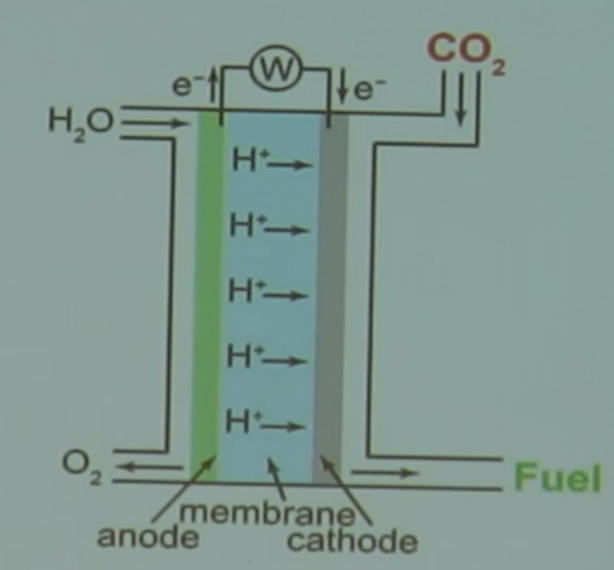
\includegraphics[width=0.3\linewidth]{echemScheme.png}
        \caption{\ce{CO2} reduction as an energy storage scheme.}
        \label{fig:echemScheme}
    \end{figure}
    \begin{itemize}
        \item Use renewable energy sources like wind and solar to drive electrochemical reactions. Specifically, driving the transfer of electrons may facilitate oxication of water to \ce{O2} at the anode reduction of \ce{CO2} to fuels (such as ethylene) at the cathode. Note that the water's protons will theoretically diffuse through a proton exchange membrane.
        \item Big idea: Store renewable intermittent electricity in energy-dense chemical bonds.
    \end{itemize}
    \item Selectivity challenges in \ce{CO2} reduction.
    \begin{itemize}
        \item One reason we don't know how to do this yet: \ce{CO2} can be reduced to myriad products.
        \item A competitive side reaction: Hydrogen evolution.
        \item Other carbonatious products include methanol, ethanol, etc. Some of these may be good, but we don't want to produce all of them at once!
        \item Though it might be theoretically possible to pin the $\Delta E$ thermodynamically, it's practially virtually impossible.
        \item Consequently, selective \ce{CO2}RR requires control over the relative rates (kinetics) of competing reactions.
    \end{itemize}
    \item Understanding of interfacial proton coupling is poor.
    \begin{itemize}
        \item \ce{CO2 + 2e^- + 2H+ -> CO + H2O} is possible.
        \item Things like molecular electrocatalysts allow us to access this at a high rate and selectivity.
        \begin{itemize}
            \item We can boost the rate even further with \emph{intra}molecular proton donors (esp. phenolic groups).
            \item \emph{Inter}molecular proton donors can help, too, but make sure not to make it too acidic, or you'll favor hydrogen evolution!
            \item Thus, what you really need is precise proton delivery.
        \end{itemize}
        \item These homogeneous catalysts are nice and pretty, but in a functional device, we'll need heterogeneous catalysis.
        \begin{itemize}
            \item Possible example: \ce{Au} catalyst.
            \item Mathematical models suggest that the concentration profiles at the interface of the solid are higher. Essentially, the $\pH$ near the surface becomes much more alkaline very quickly.
            \item We don't have control over the proton coordinate here, and we don't actually know what the proton donor is (could be water, hydronium, carbonic acid, etc.).
            \item Thus, we need to understand the role of PCET in dictating \ce{CO2}RR vs. HER selectivity.
            \item This is what Wuttig did her PhD on!
        \end{itemize}
    \end{itemize}
    \item Electrochemistry is nice because you always know the rate.
    \begin{itemize}
        \item The velocity $v$ of the reaction is related to the current $i$, the number of electrons $n$, and Faraday's constant $F=\SI{96485}{\coulomb\per mol\ e^-}$ via
        \begin{equation*}
            i = nFv
        \end{equation*}
        \item You can also measure how many product you're forming either by assuming that all current is going to your reaction, or by using in-line gas chromatography.
        \begin{itemize}
            \item In the EChem module, we'll assume that everything is going to hydrogen evolution.
        \end{itemize}
        \item Knowing how much current is going to hydrogen and \ce{CO}, we can construct a \textbf{Tafel plot}.
    \end{itemize}
    \item \textbf{Tafel plot}: The relationship that describes the log-linear dependence of the reaction rate as a function of the applied potential.
    \begin{itemize}
        \item We will take the partial current going to \ce{CO} and plot it vs. the applied potential.
        \item This yields direct mechanistic insight: Increasing the overpotential decreases the $\Delta G^\ddagger$.
    \end{itemize}
    \item Example of using a Tafel plot.
    \begin{itemize}
        \item Assume \ce{CO2} is reduced in a rate limiting step by combining with an electron.
        \item Using kinetics, we would have
        \begin{equation*}
            R_{\ce{CO}} = k_1(\theta^*)(a_{\ce{CO2}})\exp(\frac{\beta nF}{RT})
        \end{equation*}
        \begin{itemize}
            \item $\theta^*$ is the concentration of the active sites on the gold surface; not every atom on the surface is active, as can be shown via fancy microscopy techniques.
            \item $a_{\ce{CO2}}$ is the \textbf{activity} of \ce{CO2} dissolved in solution.
            \item $\beta$ is the symmetry factor: For reactions in which there is a high reorganizational potential energy, we can take $\beta\approx 1/2$.
        \end{itemize}
        \item This yields info on the Tafel slope:
        \begin{equation*}
            \pdv{\eta}{\log(j)} = \frac{\SI{60}{\milli\volt}}{\beta}
            = \SIrange{120}{150}{\milli\volt}
        \end{equation*}
        \item Thus, we check the data: At all potentials in the linear range, check for linear dependence.
        \item Tafel data implies ET RLS with slope about 1.
    \end{itemize}
    \item What if instead, we couple adsorption with proton transfer from?
    \begin{itemize}
        \item Look at the rate of \ce{CO} formation vs. the bicarbonate concentration.
        \begin{itemize}
            \item Nothing here, so it's not this.
            \item Moreover, because it's not this charged species, it's not any acidic species (because changes in one would change the $\pH$ of all).
        \end{itemize}
        \item Nothing for water, too.
        \item Thus, the data suggests that there's no proton transfer in the initial step, so it must happen afterwards.
        \item Note that changing the partial pressure of \ce{CO} also doesn't change anything, suggesting that as soon as \ce{CO} is created, it is released and future adsorption is not inhibited.
    \end{itemize}
    \item Other data complete the mechanism.
    \begin{figure}[H]
        \centering
        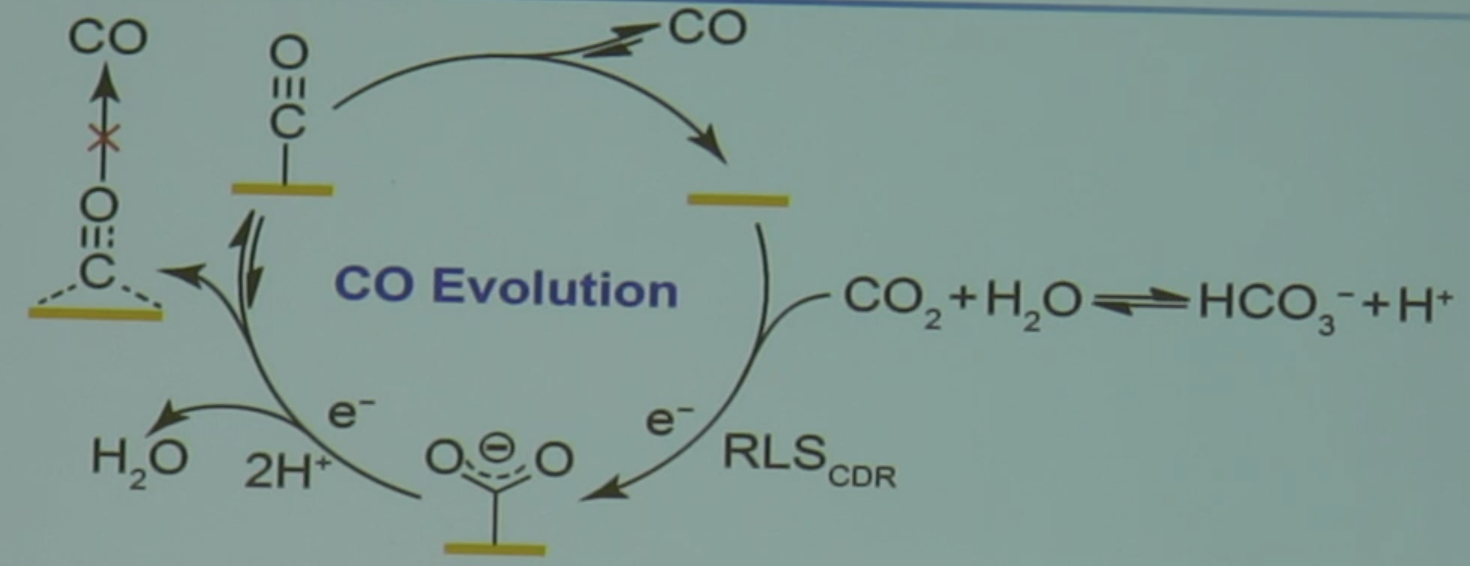
\includegraphics[width=0.5\linewidth]{COEvolution.png}
        \caption{\ce{CO} evolution mechanism.}
        \label{fig:COEvolution}
    \end{figure}
    \item Simultaneous hydrogen evolution is dependent on the proton donor environment.
    \begin{figure}[h!]
        \centering
        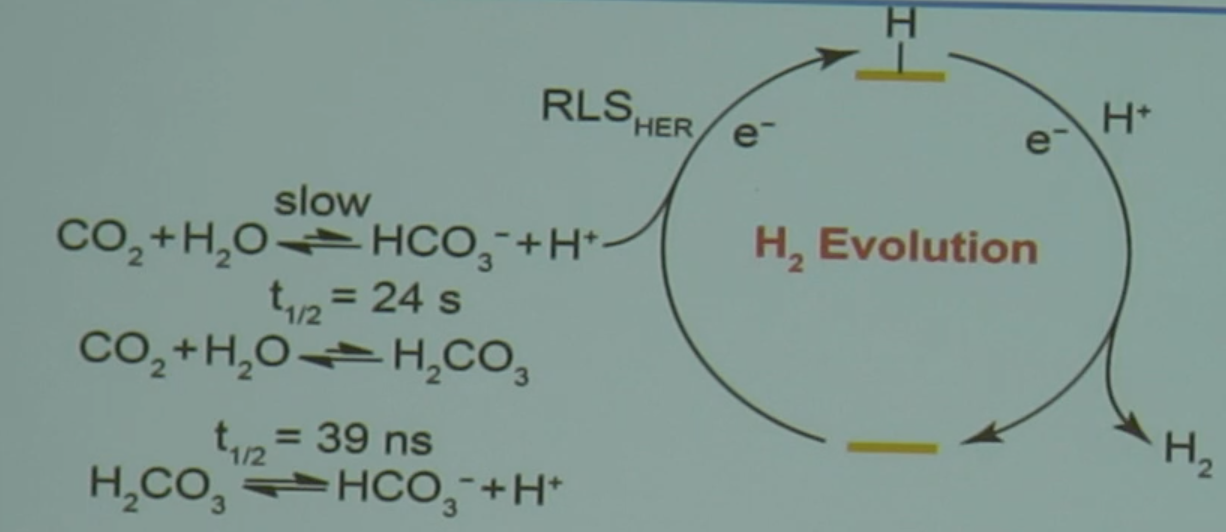
\includegraphics[width=0.5\linewidth]{H2Evolution.png}
        \caption{\ce{H2} evolution mechanism.}
        \label{fig:H2Evolution}
    \end{figure}
    \begin{itemize}
        \item Mechanism is deceptively simple, but profound all the same.
        \item We first get adsorption of a proton to a hydride.
        \begin{itemize}
            \item But Tafel slope is super high, so you may be being limited by the ability of the protons to get to the surface in the first place.
            \item Suppose that the protons are special, i.e., donated by the relatively slow dissociation of \ce{H2CO3}.
            \begin{itemize}
                \item Note that \ce{H2CO3} dissociates with $t_{1/2}=\SI{24}{\second}$ in real life; it is only super fast in our body because of an enzyme we have that takes it to $t_{1/2}=\SI{39}{\nano\second}$.
            \end{itemize}
            \item Changing the concentration of \ce{H2CO3} and rerunning the experiment confirms this.
        \end{itemize}
        \item We do observe an explicit change in the rate of hydrogen evolution based on the concentration of \ce{H2CO3}, but the relationship is complex and potential dependent.
        \item This is an independently occurring catalytic reaction on \emph{some} catalytic site (maybe one that was occupied by \ce{CO}, maybe not, we don't know).
    \end{itemize}
    \item Utilizing this mechanism to design a better, more selective reaction.
    \begin{figure}[H]
        \centering
        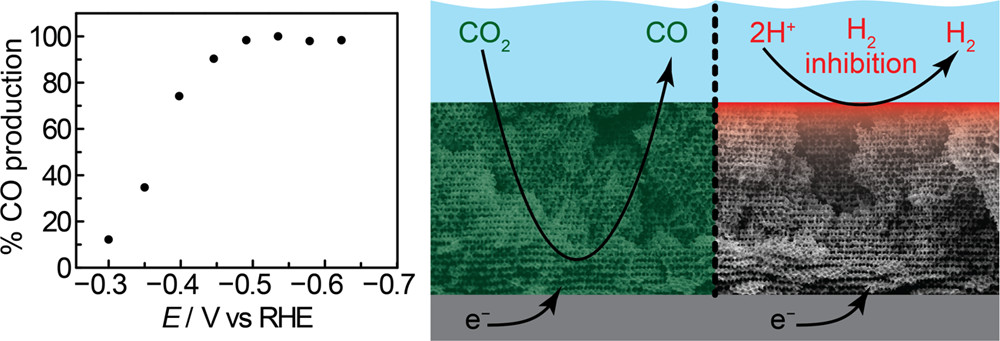
\includegraphics[width=0.5\linewidth]{mesoporousAu.jpeg}
        \caption{Enhancing heterogeneous \ce{CO2}RR with mesoporous membranes.}
        \label{fig:mesoporousAu}
    \end{figure}
    \begin{itemize}
        \item If we couple the two reactions, because they both depend on \ce{CO2 + H2O <=> HCO3- + H+}, we can increase selectivity by slowing down this equilibration even further.
        \item We make the environment at the gold catalysis further out of equilibrium with the bulk.
        \item Wuttig teamed up with other scientists to develop a mesoporous gold structure, forcing everything that wants to touch the gold to go through the structure.
        \item The \ce{CO2} reaction does not care how thick the structure is, but \ce{H2} does! This leads to near-selective \ce{CO} formation.
    \end{itemize}
    \item In our module, however, we need to \emph{increase} \ce{H2} evolution, though!
    \begin{itemize}
        \item We'll use all the same principles Wuttig just discussed, but it'll be simpler.
        \item \ce{H2} evolution is also an important reaction.
    \end{itemize}
\end{itemize}



\section{Lab 4: GCMS}
\subsection*{Lab Manual}
\begin{itemize}
    \item \marginnote{2/9:}Goal.
    \begin{itemize}
        \item Use GCMS to quantify how much benzene there is in 87 gasoline.
        \item We will use a \textbf{standard addition method} with respect to an internal standard reference.
    \end{itemize}
    \item Why we are interested.
    \begin{itemize}
        \item Gasoline is a complex mixture of hydrocarbons, and refineries are known to include aromatics such as benzene, toluene, and xylenes to increase the octane rating.
        \item However, there is increasing concern about the hazards associated with these compounds.
    \end{itemize}
    \item \textbf{Standard addition method}: The quantitation of a substance of interest in a complex mixture performed by spiking in increasing known amounts of that substance and plotting the resulting signal from this series of samples to determine the original amount.
    \item Description of how gas chromatography works.
    % \item Description of \textbf{electron ionization} and \textbf{chemical ionization} mass spectrometry.
    \item \textbf{Electron ionization} (mass spectrometry): A "hard ionization" source that results in a charged ion likely to fragment into a characteristic fragmentation pattern. \emph{Also known as} \textbf{EI}.
    \begin{itemize}
        \item As discussed in \textcite{bib:CHEM30200Notes}, electrons are generated via thermionic emission from a hot tungsten filament and then accelerated by applying a large potential between the filament and anode.
    \end{itemize}
    \item \textbf{Chemical ionization} (mass spectrometry): A "soft ionization" soruce through which the major product is the molecular ion and very little fragmentation occurs. \emph{Also known as} \textbf{CI}.
    \item EI is more useful for molecular identification against a library of known fragmentation patterns; CI is more useful for calculating the molecular weight of an unknown or newly synthesized compound.
    \item Common MS peaks in EI spectra.
    \begin{itemize}
        \item Molecular ion at $m/z=\text{MW}$.
        \item \ce{[C4H3]+} at $m/z=51$, which is often a tell-tale sign that the analyte is an aromatic.
        \item \ce{[C7H7]+} at $m/z=91$, which often arises from the rearrangement of a benzyl fragment and suggests that the analyte contains a benzyl moiety.
    \end{itemize}
    \item Mass analyzers.
    \item Methods of mass analysis: Quadrupole, time of flight, ion trap, ion cyclotron, etc.
    \begin{itemize}
        \item Our setup has both a quadrupole and time-of-flight mass analyzer.
    \end{itemize}
    \item \textbf{Quadrupole}: A device that filters out ions with very low or very high $m/z$ ratios.
    \begin{figure}[H]
        \centering
        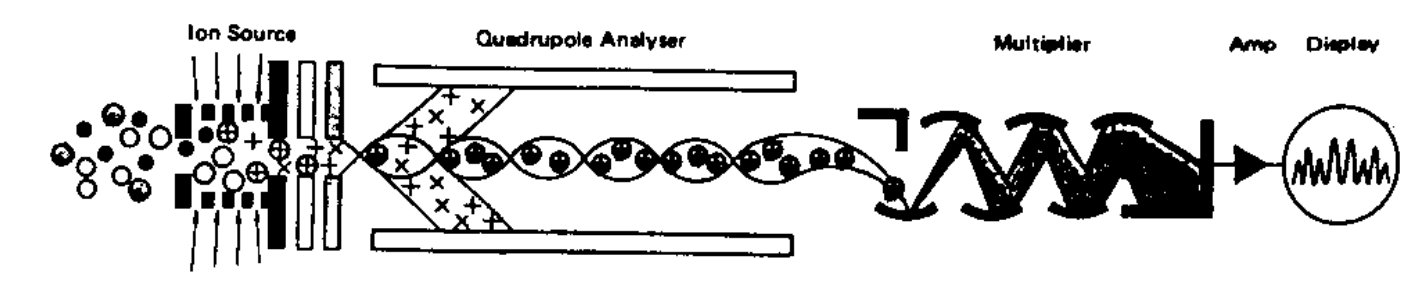
\includegraphics[width=0.7\linewidth]{quadrupole.png}
        \caption{Quadrupole mass spectrometer.}
        \label{fig:quadrupole}
    \end{figure}
    \begin{itemize}
        \item In our setup, it allows ions of our desired $m/z$ range to pass into the time-of-flight tube where they are ultimately detected.
        \item Can be tuned to scan the atomic mass range or pass only a particular mass/charge of interest.
        \item Setup: Each parallel plate contains a dc voltage as well as a radiofrequency oscillation with frequency $f$. How much something moves correlates with its mass. We use one set of plates in the $xz$-plane, and one in the $yz$-plane, each meant to filter out an extreme of mass.
    \end{itemize}
    \item \textbf{Time of flight}: A device that accelerates charged particles along a path and measures how long they are in the tube before they crash into a detector. \emph{Also known as} \textbf{TOF}.
    \begin{figure}[h!]
        \centering
        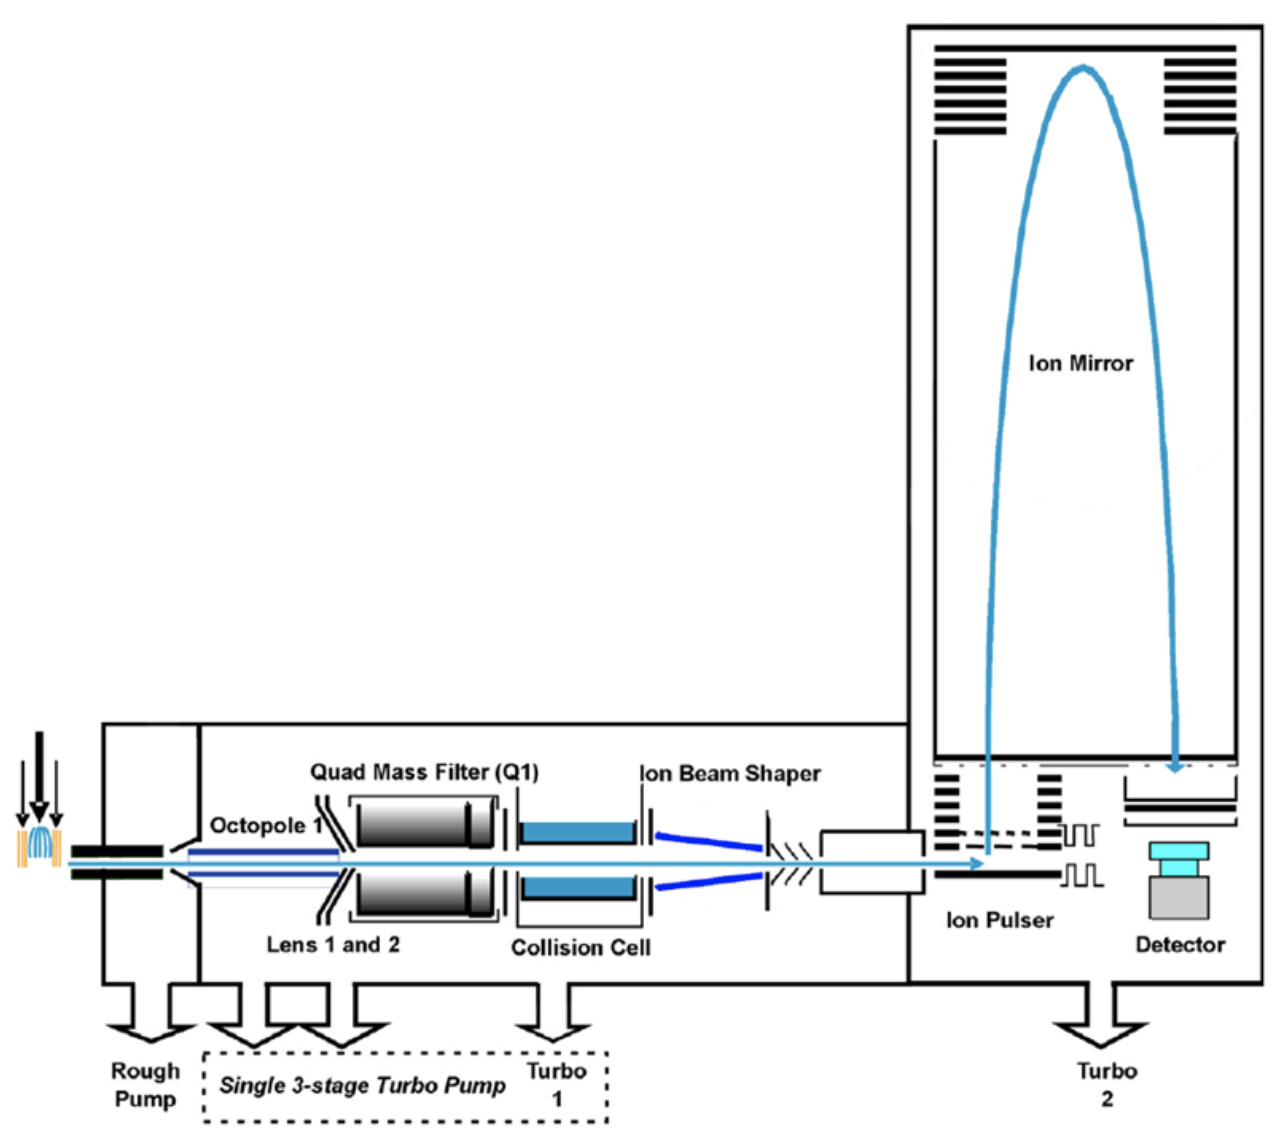
\includegraphics[width=0.6\linewidth]{TOF.png}
        \caption{Time of flight mass spectrometer.}
        \label{fig:TOF}
    \end{figure}
    \begin{itemize}
        \item We rearrange $E=(1/2)mv^2$ to
        \begin{equation*}
            m = \left( \frac{2E}{d^2} \right)t^2
        \end{equation*}
        \item Smaller ions are accelerated to a higher total velocity and arrive at the detector first.
    \end{itemize}
    \item Standard addition analysis: Largely to be discussed in lab.
    \item Error analysis discussed.
\end{itemize}


\subsection*{In Lab}
\begin{itemize}
    \item We are not actually solving the linear fit for concentration, but for the added concentration. This will be negative since we're concentrating the amount you would have to remove in order for the peak to disappear, which is the opposite of the initial amount.
    \item Using an internal standard allows us to divide out volume.
    \begin{itemize}
        \item Let \ce{R} denote the substance of interest.
        \item We have that
        \begin{equation*}
            A_{\ce{R}} \propto [\ce{R}]
            = V\cdot\eta_{\ce{R}}\cdot[\ce{R}]
            = V\cdot\eta_{\ce{R}}\cdot([\ce{R}]_0+[\ce{R}]_\text{add})
        \end{equation*}
        where\dots
        \begin{itemize}
            \item $A_{\ce{R}}$ is the GC peak area.
            \item $V$ is the sample volume.
            \item $[\ce{R}]$ is the concentration of $R$.
            \item And $\eta_{\ce{R}}$ is the detector efficiency for \ce{R}.
        \end{itemize}
        \item Thus, there will be a linear relationship between $[\ce{R}]_\text{add}$ and $A_{\ce{R}}$, the $x$-intercept of which occurs when $[\ce{R}]_\text{add}=-[\ce{R}]_0$.
        \item When $V$ is nonconstant (there will be slight variations in how much sample we add to the GCMS tube each time), we can use an \textbf{internal standard} to correct our work.
        \item In particular, if \ce{B} denotes benzene and \ce{T} denotes toluene, we have
        \begin{align*}
            A_{\ce{B}} &= V\cdot\eta_{\ce{B}}\cdot([\ce{B}]_0+[\ce{B}]_\text{add})&
            A_{\ce{T}} &= V\cdot\eta_{\ce{T}}\cdot[\ce{T}]_0
        \end{align*}
        \item We can then divide these two equations to obtain
        \begin{align*}
            \frac{A_{\ce{B}}}{A_{\ce{T}}} &= \frac{\eta_{\ce{B}}}{\eta_{\ce{T}}}\cdot\frac{[\ce{B}]_\text{add}}{[\ce{T}]_0}+\frac{\eta_{\ce{B}}}{\eta_{\ce{T}}}\cdot\frac{[\ce{B}]_0}{[\ce{T}]_0}\\
            &= \frac{\eta_{\ce{B}}}{\eta_{\ce{T}}\cdot[\ce{T}]_0}\cdot([\ce{B}]_\text{add}+[\ce{B}]_0)
        \end{align*}
        \begin{itemize}
            \item Notice that $V$ cancels out!
        \end{itemize}
    \end{itemize}
    \item \textbf{Internal standard}: A substance in a solution that is always at the same concentration.
    \item These last two points are related to Q3-4 of the lab report.
    \item 0,2.5,5,7.5,10,12.5 are data points.
    \item \textbf{Extract chromatogram} allows you to find all peaks that have a significant concentration of a certain $m/z$.
    \begin{itemize}
        \item For example, you can type in $m/z=78$ and find all peaks corresponding to benzene (there should only be one).
        \item $m/z=91$ will get you all toluene derivatives.
        \begin{itemize}
            \item Xylenes come in a pair of three (ortho/meta/para).
        \end{itemize}
        \item $m/z=105$ should yield all xylene derivatives.
    \end{itemize}
    \item Range of masses: 50-600; Solvent pause time: 4 min.
    \item 0ppm.
    \begin{itemize}
        \item Rt: 4.696. Benzene. Integration: 321274.63.
        \item Rt: 6.858. Toluene. Integration: 329835.47.
        \item Rt: 8.540. \emph{para}-Xylene. Integration: 353207.99.
        \item Rt: 8.363. Ethyl benzene. Integration: 104551.1.
        \item We're now using mesitylene instead of \emph{para}-xylene.
    \end{itemize}
    \item Notes on how to answer the questions.
    \begin{enumerate}
        \item Input 0ppm data in to Excel. Plot the regular chromatagram (TIC) vs. retention time.
        \item Plot an EIC for both benzene and toluene. Also plot their extracted mass spectra (peak labels [3-4 per spectrum] should include a name or structure and an $m/z$ value). This can be extracted from the 0ppm data as well.
        \item Using integration data for both benzene and toluene at all concentrations (jotted down) and ppm data (given), normalize the benzene data using the toluene data (toluene is an \textbf{internal standard} because it's always at the same concentration, so it makes benzene peaks comparable via normalization), make a scatter plot, find the line of best fit, and calculate the concentration.
        \item Use the Student's $t$-test, 95\% confidence interval, $n-2=3$ DOFs, to get $t=3.182$. No need to cite a source. For tabulation, make a very simple $2\times 2$ table with headers "Concentration" and "Error" and then place the values below. To get a volume percentage, use HL's Canvas announcement to convert concentration in ppm (not mol/L) to a mass percentage, and then a volume percentage (using density).
        \begin{itemize}
            \item Hypothetical: Imagine 1 gram of solution (approximate as pentane density). You can convert it to liters pentane using the density and stoichiometry.
            \item Now imagine you have \SI{5}{\micro\gram} benzene. You can convert it to liters benzene using the density and stoichiometry.
            \item Divide the latter by the former to obtain a volume percentage.
        \end{itemize}
        \item Plot EICs and MSs for both mesitylene and ethyl benzene. The EICs can be the same in both cases. Peak areas are comparable across EICs, so just compare the peak area of benzene which correlates with it's above-derived concentration to estimate the concentrations of mesitylene and ethyl benzene using a simple ratio.
    \end{enumerate}
\end{itemize}




\end{document}